\documentclass[12pt]{article}

\usepackage{graphicx}
\usepackage{amsmath}
\usepackage{amssymb}
\usepackage{natbib}
\usepackage{amsfonts}
\usepackage{multicol}
\usepackage{float}
\usepackage{oldgerm}
\usepackage{bm}
\usepackage{mathtools}
\usepackage{wrapfig}
\usepackage{fancyhdr}
\usepackage[export]{adjustbox}
\usepackage{xcolor}
\usepackage[shortlabels]{enumitem}

\pagestyle{empty}

\setlength{\headsep}{0.5cm}
\setlength{\oddsidemargin}{-0.5cm}
\setlength{\textwidth}{16.5cm}
\setlength{\textheight}{24cm}
\voffset = -2cm


\pagestyle{fancy}
\fancyhf{}
\rfoot{
\includegraphics[width=1.0in]{cnm.png}}
\lfoot{Homework 2}
\setlength\parindent{0pt}
\begin{document}

\begin{center}
\hfil
{\large\bf {ENGR 2910-101: Circuit Analysis}}
\hfill Instructor: Brian Rashap\\
Homework 2: 01/18/23 \hfill Due: 01/25/23\\
\hrulefill\\
\end{center}

{\bf Question 1} [10] %2.14

The terminal voltage and terminal current were measured (b) on the device (a) shown. Construct a circuit model for the device consisting of a single resistor. Provide a graph (either hand-drawn or software generated) showing how you determine the value of the resistor. 

\begin{figure}[h!]
\centering 
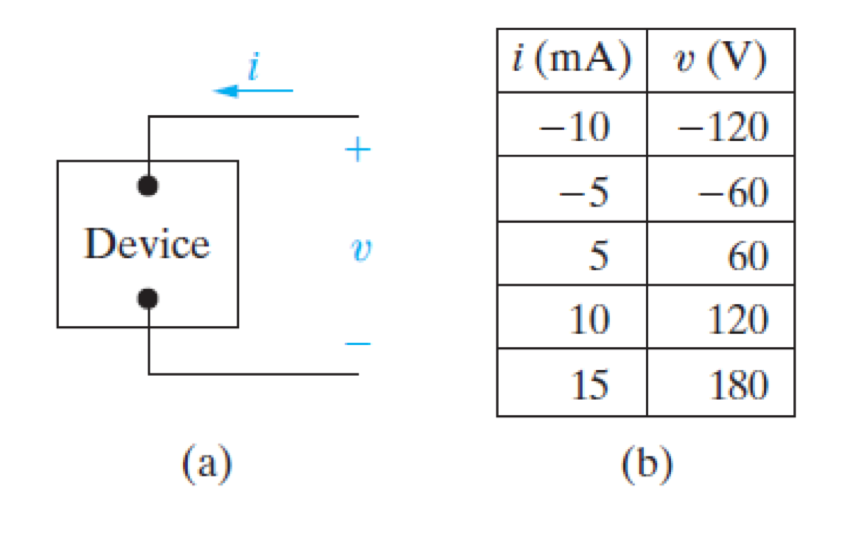
\includegraphics[clip,width=0.49\textwidth]{P2-14.png}
\end{figure}

{\bf Question 2} [10] %2.18

\begin{figure}[h!]
  \centering 
 \vspace{-0.1in}
 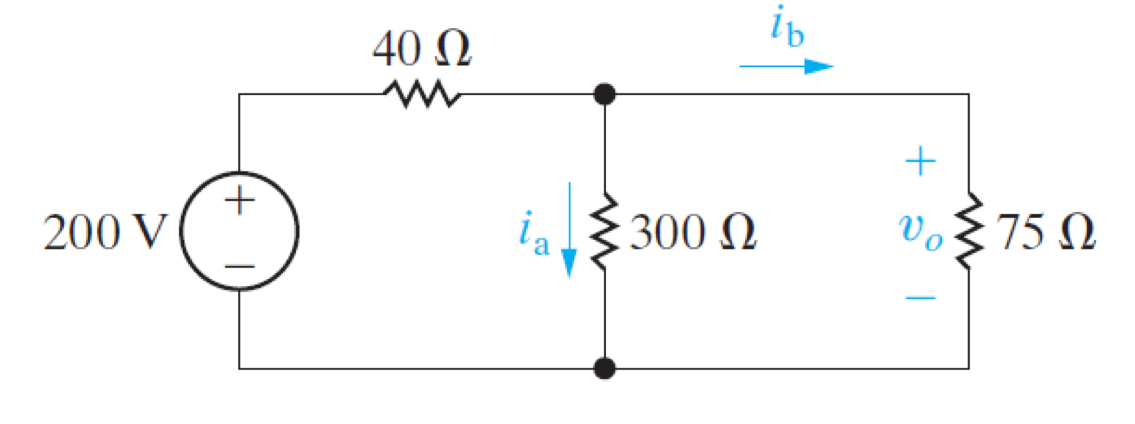
\includegraphics[clip,width=0.7\textwidth]{Fig2-18.png}
\vspace{-0.1in}
\end{figure}

For the circuit shown, find: 
\begin{enumerate}[(a)]
\item The value of $i_a$.
\item The value of $i_b$.
\item The value of $v_a$.
\item the power dissipated in each resistor.
\item the power delivered by the $200V$ source.
\end{enumerate}

\newpage
{\bf Question 3} [10] %P2-22

In the circuit below, the current $i_{o} = 2A$.  
\begin{figure}[h!]
     \centering
\vspace{-0.1in}
     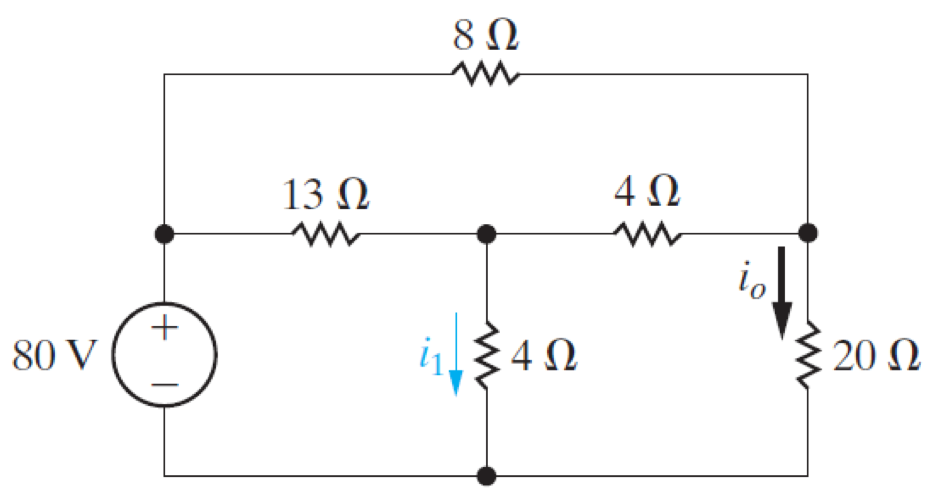
\includegraphics[clip,width=0.6\textwidth]{Fig2-22.png}
\vspace{-0.15in}
\end{figure}

\begin{enumerate}[(a)]
\item Find $i_1$.
\item Find the power dissipated in each resistor.
\item Verify that the total power dissipated in the circuit equals the power provided by the voltage source.
\end{enumerate}

{\bf Question 4} [10] %P2-27

The variable resistor $R$ is adjusted until $i_{o} = 10$ mA. Find the value of $R$.
\begin{figure}[!h]
  \centering 
  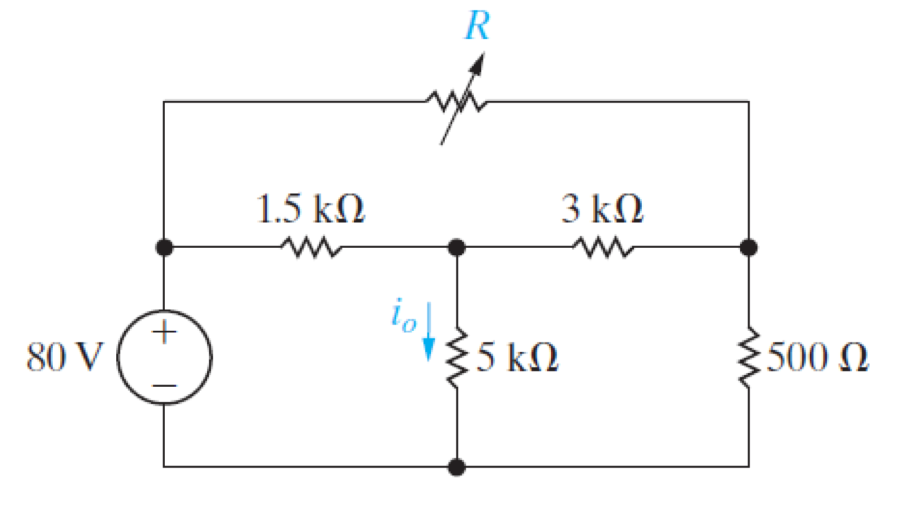
\includegraphics[clip,width=0.6\textwidth]{Fig2-27.png}
\end{figure}

{\bf Question 5} [10] %P2-34

Find $v_{o}$ and the total power supplied in the circuit.
\begin{figure}[h!]
\centering 
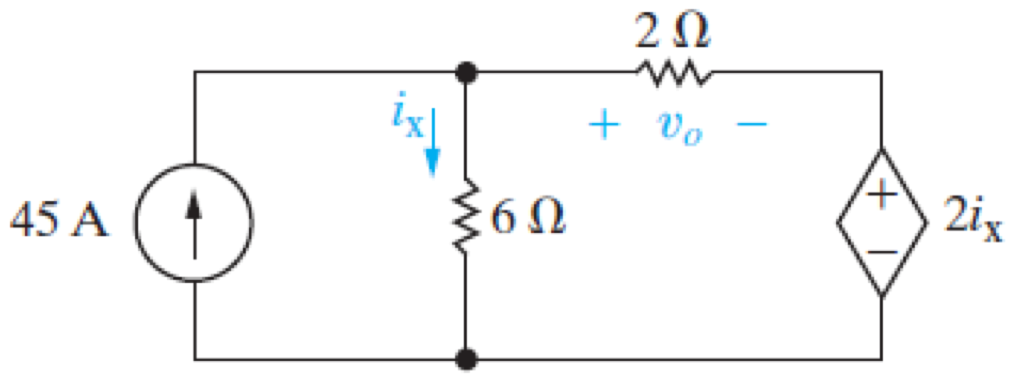
\includegraphics[clip,width=0.6\textwidth]{Fig2-34.png}
\end{figure}


\end{document}
